%************************************************
\chapter{Introduction to Learning-to-Rank}
Different definitions of Learning-to-Rank exist. In general, all ranking methods that use machine learning technologies to solve the problem of ranking are called Learning-to-Rank methods. Figure \ref{fig:discriminative_training} describes the general process of machine learning. It shows training elements from an input space that are mapped to an output space using a model such that the difference between the actual labels of the training elements and the labels predicted with with the model are minimal in terms of a loss function.
\begin{figure}[!h]
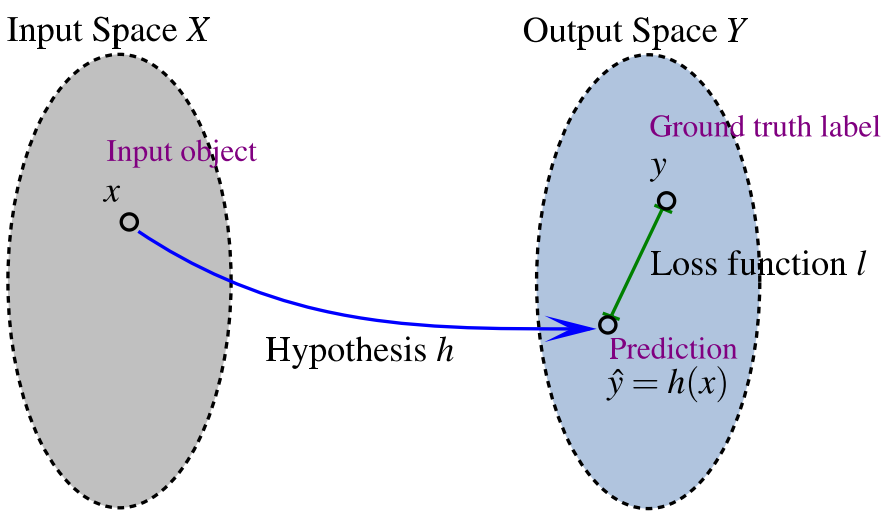
\includegraphics[scale=0.26]{gfx/descriminative_training}
\caption{Machine learning framework for Learning-to-Rank, obtained from Liu\cite{Liu2007}}
\label{fig:discriminative_training}
\end{figure}\\
Liu \cite{Liu2007} proposes a more narrow definition and only considers ranking methods to be a Learning-to-Rank method when it is \emph{feature based} and uses \emph{discriminative training}, which are itself defined as follows:
\begin{description}
\item[Feature Based]{\emph{Feature based} means that all documents under investigation are represented by feature vectors that reflect the relevance of the documents to the query.}
\item[Discriminative Training]{\emph{Discriminative training} means that the learning process can be well described by the four components of discriminative learning. That is, a Learning-to-Rank method has its own \emph{input space}, \emph{output space}, \emph{hypothesis space}, and \emph{loss function}, like the machine learning process described by Figure \ref{fig:discriminative_training}. \emph{Input space}, \emph{output space}, \emph{hypothesis space}, and \emph{loss function} are hereby defined as follows:
	\begin{description}
	\item[Input Space]{contains the objects under investigation. Usually objects are represented by feature vectors, extracted according to different applications.}
	\item[Output Space]{contains the learning target with respect to the input objects.}
	\item[Hypothesis Space]{defines the class of functions mapping the input space to the output space. The functions operate on the feature vectors of the input object, and make predictions according to the format of the output space.}
	\item[Loss Function]{in order to learn the optimal hypothesis, a training set is usually used, which contains a number of objects and their ground truth labels, sampled from the product of the input and output spaces.}
	\end{description}
	}
\end{description}


Figure \ref{fig:ltr_framework} shows how the machine learning process as described in Figure \ref{fig:discriminative_training} typically takes place in a ranking scenario. A set of queries $q_i$ with $n > i > 1$, the documents associated with these queries which are represented by feature vector $x_i$, and the relevant judgements of those documents $y_i$ are used together to train a model $h$, that can predict a ranking of the documents $y_i$, such the difference between the document rankings predicted by $h$ and the actual optimal rankings based on $y_i$ is are minimal in terms of a loss function.
\begin{figure}[!h]
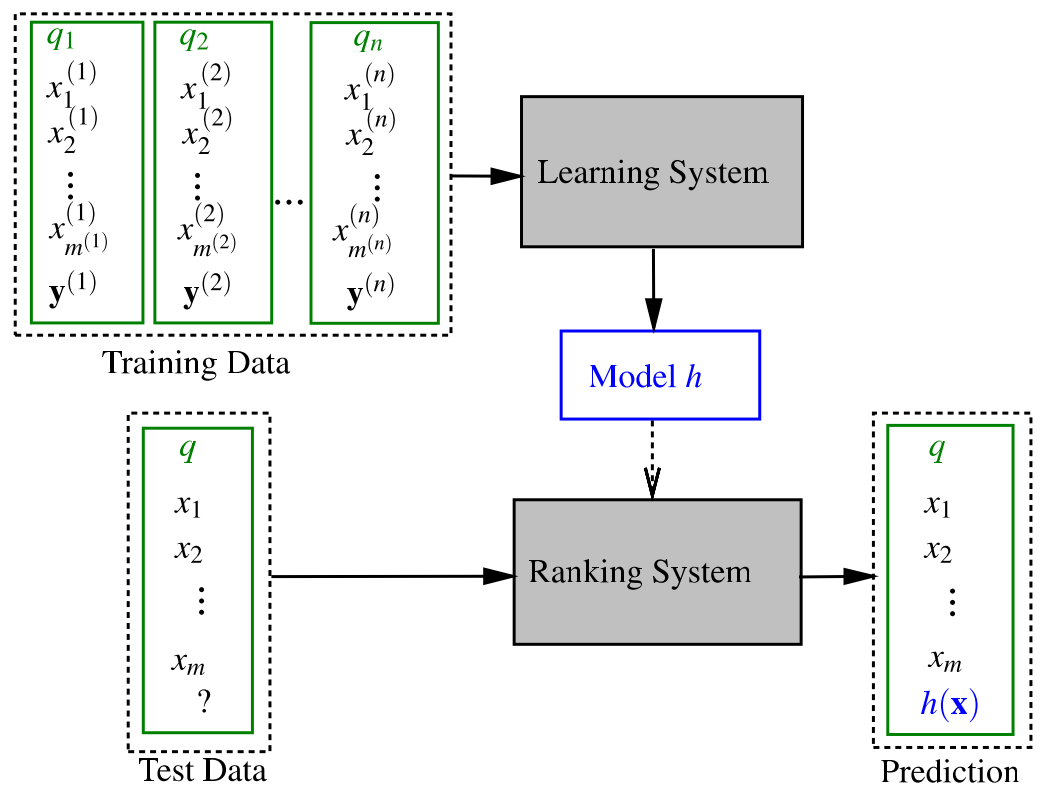
\includegraphics[scale=0.25]{gfx/ltr_framework}
\caption{A typical Learning-to-Rank setting, obtained from Liu\cite{Liu2007}}
\label{fig:ltr_framework}
\end{figure}\\

The predictions and the loss function might either be defined for:
\begin{enumerate}
\item the relevance of a single document
\item the classification of the most relevant document out of a document-pair
\item the ranking of documents directly
\end{enumerate}
These three approaches are in literature respectively called the pointwise approach, the pairwise approach and the listwise approach. In the following sections we will further describe the three different approaches in Learning-to-Rank.

\section{Pointwise Approach}

\section{Pairwise Approach}
\section{Listwise Approach}
\chapter{Evaluation Methods}

\section{Normalized Discounted Cumulative Gain}
Cumulative gain, or its predecessor discounted cumulative gain and normalized discounted cumulative gain, is one of the most widely used measures for effectiveness of ranking methods.
\subsection{Discounted Cumulative Gain}
The \ac{DCG}\cite{Burges2005} at a position $p$ is defined as\\
$DCG_p = \sum\nolimits_{i=1}^p \frac{2^{rel_i-1}}{log_2(i+1)}$\\
with $rel_i$ the graded relevance of the result at position $i$. The idea is that highly relevant documents that appear lower in a search result should be penalized (discounted). This discounting is done by reducing the graded relevance  logarithmically proportional to the position of the result.
\subsection{Normalized Discounted Cumulative Gain}
\ac{nDCG} normalizes the \ac{DCG} metric to a value in the [0,1] interval by dividing by the \ac{DCG} value of the optimal rank. This optimal rank is obtained by sorting documents on relevance for a given query. We can write the definition of \ac{nDCG} down mathematically as\\
$nDCG_p = \frac{DCG_p}{IDCG_p}$
\section{Expected Reciprocal Rank}
\ac{ERR}\cite{Chapelle2009} was designed based on the observation that \ac{nDCG} is based on the false assumption that the usefulness of a document at rank $i$ is independent of the usefulness of the documents at rank less than $i$. \ac{ERR} is based on the reasoning that users are likely to stop exploring the result list once they have found a document that satisfied their information need. The \ac{ERR} metric is defined as the expected reciprocal length of time that the user will take to find a relevant document. \ac{ERR} is formally defined as\\
$ERR = \sum\nolimits_{r=1}^n \frac{1}{r} \prod\nolimits_{i=1}^{r-1}(1-R_i)R_i$\\
where the product sequence part of the formula represents the chance that the user will stop at position $r$.\\
An algorithm to compute \ac{ERR} is shown in Listing \ref{lst:err}. The algorithm requires relevance grades $g_i$, $1 \le i \le n$ and mapping function $R$ that maps relevance grades to probability of relevance.
\begin{lstlisting}[caption={Algorithm to compute the ERR metric, obtained from \cite{Chapelle2009}}, label={lst:err},language=Ada]
p <- 1, ERR <- 0
for r=1 to n do
	R <- R(g[r])
	ERR <- ERR + p * R/r
	p <- p * (1-R)
end for
return ERR
\end{lstlisting}
\section{Mean Average Precision}
\ac{AP}\cite{Zhu2004} is an often used binary relevance judgement based metric that can be seen as a trade-off between precision and recall that is defined as\\
$AP = \frac{\sum\nolimits_{k=1}^{n}Precision(k)*relevance(k)}{\text{number of relevant docs}}$\\
With $k$ being the positions in the result set between 1 and $n$.
\ac{MAP} is the average \ac{AP} for a set of queries.\\
$MAP = \frac{\sum\nolimits_{q=1}^{Q}AP(q)}{Q}$